\documentclass{article}
\usepackage[utf8]{inputenc}
\usepackage{graphicx}
\graphicspath{ {images/}}
\usepackage{amsthm}
\usepackage{amssymb}
\usepackage{amsfonts}
\usepackage{color}
\usepackage{colortbl}
 \usepackage{wrapfig}
\usepackage{enumitem}
\usepackage{hyperref}
\title{TP 4 \\ Arithmétique}
\author{SABABADY Kamala et SELVARAJAH Dinusan}

\begin{document}
\maketitle

\section{{\color{red}Partie 1 :}  \textit{Un nombre est-il premier ?}}

Soit a un nombre entier et b un nombre entier non nul. La division euclidienne de a par b est l'opération qui associe à a et à b deux nombres entiers q et r définie par : a = b $*$ q + r avec r $<$ b.
En Python, le quotient et le reste de la division euclidienne d'un entier par un entier s'obtient de la façon suivante: pour le quotient on utilise a/b et pour le reste on cherche son modulo ($a\%b$).

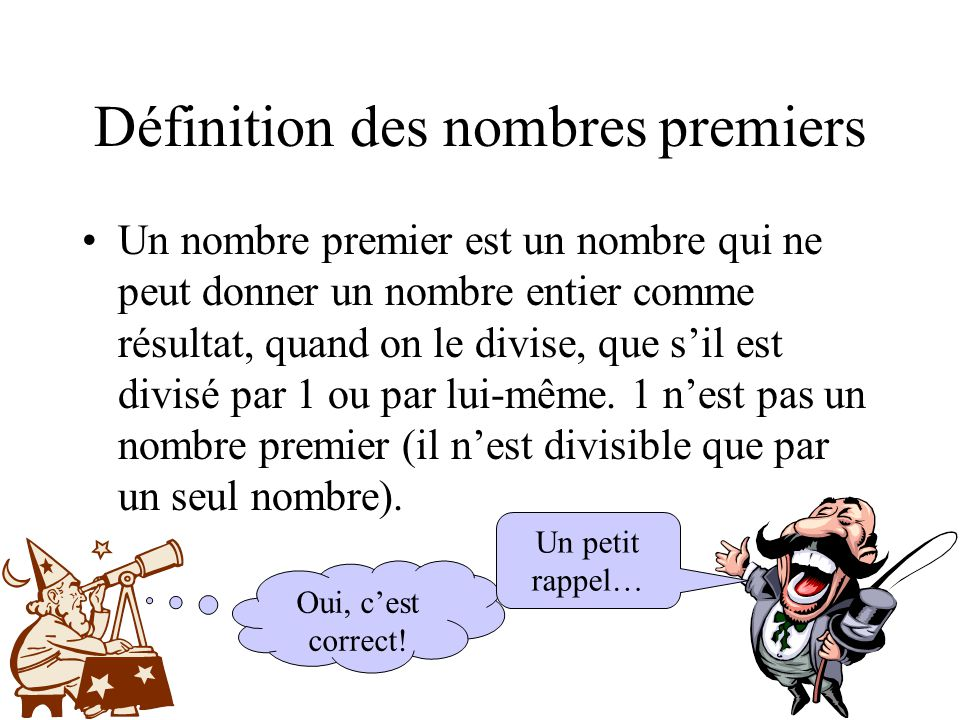
\includegraphics[width=9cm]{10.jpg}
\\

Prenons les exemples données dans la consigne et vérifions s'ils sont premiers ou pas :\\
 $1001 = 11 * 91$ donc il n'est pas premier.\\
 $2017$ est un nombre premier.\\
 $3001$  est un nombre premier.\\
 $49999$ est un nombre premier.\\
 $89999 = 7*12857$ donc il n’est pas premier.\\

Nous avons défini une fonction python \textit{is\_prime} qui prend un argument un entier n et qui renvoi \textit{true} si n est premier, \textit{false} sinon.

Les nombre de Fermat $F_0,F_1,F_2,F_3,F_4$ sont premier mais $F_5$ n'est pas premier. 


\section{{\color{red}Partie 2 :} \textit{Crible d'Erasthotène, distribution des nombres premiers.}}

\begin{wrapfigure}{l}{0.25\textwidth}
\centering
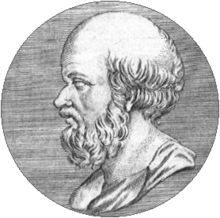
\includegraphics[width=0.25\textwidth]{01.png}
\end{wrapfigure}
$$ $$
\textit{"ÉRATOSTHÈNE de Cyrène est un astronome, géographe et mathématicien, nommé à la tête de la bibliothèque d'Alexandrie, il est resté célèbre pour son crible et pour avoir le premier mesuré le méridien terrestre."}
\\
\\
$$ $$
	On cherche des nombres premiers à l'aide du Crible d'Erathostène.\\
Voici les entiers naturels de 1 à 200:
\\
\\

\input{"table.txt"}\\
\\

Nous avons obtenu ce tableau en éliminant :
\begin{itemize}[label=\textbullet, font=\LARGE \color{black}]
\item 1 qui n'est pas un nombre premier donc {\color{red}\textbf{la case}} est coloriée en rouge.
\item Tous les {\color{red}multiples de 2} excepté \textbf{2}
\item Tous les {\color{cyan}multiples de 3} excepté \textbf{3}
\item Tous les {\textbf{\color{yellow}multiples de 5}} excepté \textbf{5}
\item Tous les {\color{green}multiples de 7} 
\item Tous les {\color[RGB]{255,0,186}multiples de 11}
\item Tous les {\color[RGB]{150,0,186}multiples de 13}
\end{itemize}
$$ $$
Pour les nombres premiers inférieurs à 200 on a tous les nombres restants en gras.

La fonction \texttt{primes} qui prend en argument un entier $n$ et qui renvoie la liste de tous les premiers inférieurs à $n$ est créée en faisant le test de chaque entier inférieur à cet entier n avec la fonction \textit{is\_prime} qu'on a vu précédemment et voir si l'entier est inférieur , si c'est le cas on l'enregistre dans une liste . 

On a ensuite créée cette liste pour tous les premiers inférieurs à 1000 avec la fonction \texttt{primes} et nous l'avons enregistré dans un fichier texte primes.txt.

$$ $$
\input{"primes.txt"}
$$ $$
On a défini une fonction $\pi(n)$ le nombre d'entiers premiers inférieurs à $n$ , pour la définir on a appliqué la fonction \texttt{primes} à n et puis on calcule la longueur de la liste que l'on retourne. 
\\
Voici le graphique avec $\pi(n)$ en fonction de $n$ pour $n$ variant de $2$ à $1000$ (courbe rouge), dans ce même graphique nous avons rajouté la fonction $g(n) = \frac{n}{\log n}$ (courbe bleu):

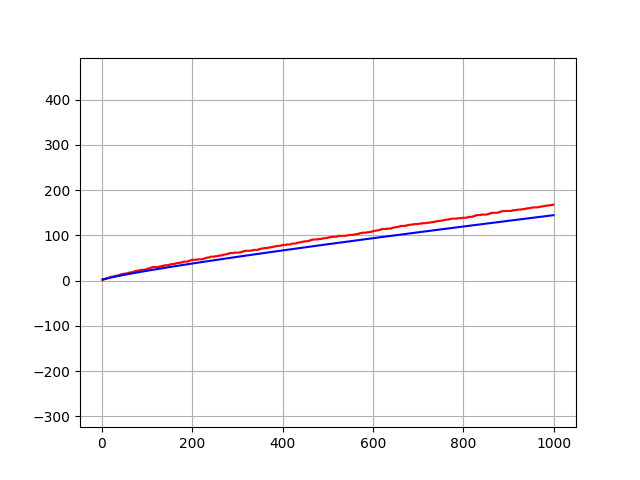
\includegraphics[width=0.85\textwidth]{graph.png}
$$ $$

On observe que la fonction $g(n)$ est proche de la courbe $\pi(n)$ donc des nombres premiers inférieur à N c'est-à-dire ici $1000$.
$$ $$
Voici la table suivante des deux fonctions $\pi(n)$ et $g(n)$ pour n allant de 10 à 1000000 :

\begin{center}
\begin{tabular}{r | c | c}
$n$ & $\pi(n)$ & $\frac{n}{\log n}$ \\
\hline
$10^1$ & {4} & {4.34294}\\
$10^2$ & {25} & {21.7147}\\
$10^3$ & {168} & {144.765}\\
$10^4$ & {1229} & {1085.74}\\
$10^5$ & {9592} & {8685.89}\\
$10^6$ & {78498} & {72382.4}
\end{tabular}
\end{center}
 On remarque que plus n est grand plus l'approximation est précise comme l'on observe sur le graphique.

\section{{\color{red}Partie 3 :} \textit{Factorisation d'un entier en premiers.}}

Le théorème fondamentale de l'arithmétique dit que tout entier positif peut être écrit sous forme d'un produit de nombres premiers, et cette décomposition est unique, à l'ordre près des facteurs.

La décomposition en facteurs premiers de $924$ est : $924 = 2*2*3*7*11$\\

On a défini deux fonctions de deux manières différentes sur Python \texttt{factors} et \texttt{factors1}, les deux fonctions donnent le même résultat. Nous avons testé avec les nombres 924 et 60. Par exemple pour la fonction \texttt{factors1} qui prend en argument un entier n et qui renvoi la liste dans l’ordre croissant des facteurs premier de n , on a réalisé des divisions successives de n par les nombres premiers qui lui sont inférieurs .
A chaque fois que n est divisible par un nombre premier on l’enregistre dans la liste puis on passe au suivant. Nous avons testé cette fonction pour $60$ et on a obtenu [$2,2,3,5$]

\section{{\color{red}Partie 4 :} \textit{PGCD de deux entiers, identité de Bézout, algorithme d’Euclide.}}

Le PGCD est le plus grand commun diviseur de 2 entiers. Soit a et b deux entiers naturels , le PGCD de a et b est le plus grand des diviseurs communs de a et b.

En utilisant la décomposition en facteurs premiers on a pour le pgcd de a = 4864 et b = 3458 :\\
\\
$a = 4864 = 2*2*2*2*2*2*2*2*19 = 28*19$
\\
$b = 3458 = 2*7*13*19$
\\
$pgcd(4864 ; 3458) = 2*19 = 38$

$$ $$

L'énoncé de L'identité de Bézout est la suivante : \\
\textit{"Soient a et b deux entiers relatifs et d leur PGCD alors il existe deux entiers u et v tels que a·u + b·v = d."}
\\
A l'aide de l'\href{https://en.wikipedia.org/wiki/Extended_Euclidean_algorithm}{algorithme d'Euclide étendu} , on calcule le pgcd de 4864 et 3458 :\\
\\
$4867 = 1 * 3458 + 1406$\\
$3458 = 2 * 1406 + 646$\\
$1406 = 2 * 646  + 114$\\
$646  = 5 * 114  + 76$\\
$114  = 1 * 76   + 38$\\
$76   = 2 * 38   + 0$\\

Donc le $pgcd(4864,3458) = 38$.
\\
\\
Pour obtenir les coefficient de Bézout, il suffit de remonter l'algorithme d'Euclide à l'envers :\\
\\
$1406 = 4864 - 3458$\\
$646  = 3458 - 2 * 1406$\\
$114  = 1406 - 2 * 646 $\\
$76   = 646  - 5 * 114$\\
$38   = 114  - 76$\\

Puis on remplace successivement :\\
	$38 = 114 – 76$ \\
	$38 = 114 – (646 – 5*114)$ \\
	$38 = - 646 + 6 * 114$\\
	$38 = -646 + 6 * (1406 – 2 * 646)$\\
	$38 = 6 * 1406 – 13 * 646$\\
	$38 = 6 * 1406 – 13 * (3458 – 2 * 1406)$\\
	$38 = 32 * 1406 – 13 * 3458$\\
	$38 = 32 * (4864 – 3458) – 13 * 3458$\\
	$38 = 32 * 4864 – 45 * 3458$\\
On trouve ainsi les coefficients de Bézout x et y avec $x = 32$ et $y = -45$.
\\

Nous avons défini une fonction \texttt{euclide} qui prend en arguments deux entiers $a, b$ et qui renvoie $x, y, d$, où $d$ est le pgcd de $a, b$ et $x, y$ les coefficients de Bézout.
On le teste pour 4864 et 3458 et on obtient bien $d = 38$ , $u = 32$ et $v = -45$


\end{document}

